\chapter{Results}
\label{cha:results}


This chapter discusses the basic findings of the analysis of the proposed peer influence model.
All results were obtained from synthetic networks which were generated over \( T = 75,000 \) iterations.
The size of the networks was fixed to \(n = 5,000 \) nodes and since the model heavily depended on events that happen at random are the reported properties of the time-varying networks obtained by averaging the results of 40 independent runs.
The model parameter which are responsible for the formation of the community structures are set to \( p_{\Delta} = 0.90 \) for the triadic closure probability, \( \delta = 1 \) for the link reinforcement constant, and \( p_{d} = \num{5e-05} \) for the node deletion probability for every experiment.
Furthermore, the critical peer influence threshold was fixed to \( \theta = 0.10 \).
This reflects the idea that only a relatively small number of active neighbors is sufficient to increase the activity of a node in a significant way.

The time-dependent topological properties of the integrated network, which are discussed in \cref{sec:integrated-network-properties}, are measured only for nodes that are part of the temporal network.
This means that nodes which were removed earlier due to the node deletion process do not influence the properties of the integrated network any more.
\Cref{sec:network-activity} contains an overview of the overall network activity with respect to different levels of peer influence.
The effect of the peer influence mechanism on the inter-event time distribution in the network is examined in \cref{sec:inter-event-time-dists}.
All this experiments are performed for different values for the maximum peer influence probability \( q \).
However, the analysis performed in the last section (\cref{sec:softmax-rescaling}) uses a fixed value for the peer influence level and discusses how different values for \( \beta \), the inverse temperature for the softmax weight re-scaling, changes the peer influence effects in the network.
The synthetic networks which are used in the first three sections adopt the average tie strength as temperature for the softmax weight re-scaling.
Therefore, \( \beta \) is set to the to the inverse of the average of the weights in the integrated network in each iteration after the first one (i.e., \( \beta = 1 \) in the initial round to avoid division by zero, since no ties have been formed yet).


%% ========================================================================
%% ========================================================================


\section{Time-dependent Integrated Network Properties}
\label{sec:integrated-network-properties}

Not only the integrated network of all 75,000 previous instantaneous networks and its properties are of great interest, but also how they evolve during the simulation.
This allows to get a deeper understanding on how the model shapes the community structures in the network and the role of peer influence on it.
To make this possible is the integrated network build in an iterative fashion.
A snapshot of it is taken after the newly formed ties are added and the weights of already established links are updated in every time step.
Features like the average local clustering coefficient or the average weight of the ties are calculated for all of the 75,000 integrated network snapshots.
This allows to examine on how the topology and other measures change over time.

The first, and most interesting, measure that can be investigated in this way is the average local clustering coefficient \( C(t) \).
\Cref{fig:avg-local-cc-full} depicts the development of it over the course of the simulation for different levels of peer influence.
The graph of this function has a very distinctive pattern, which was already explained in the original work by \citet{Laurent2015}.
The average clustering coefficient is very small in the first few hundred iterations, due to the sparsity of the integrated network.
Almost all nodes are disconnected and the number of triangles which have formed is relatively small compared to the size of the network.
However, \cref{fig:avg-local-cc-full} also shows that the clustering coefficient grows very fast until it reaches its maximum value.
This rapid increase is caused by the cyclic closure mechanism of the model.
Nodes that become active in this early stage first have to introduce some ties with nodes which are selected using the focal closure mechanism.
This does not increase the average local clustering coefficient in a significant way, however, it establishes the egocentric networks.
After the first triangles are closed, the first strong ties start to develop.
These emerging strong ties amplify the biased local search of the triadic closure mechanism and result, on one hand, in in more triangles, and on the other hand, in the reinforcement of already established triangles and the associated strong ties.
This leads to a high local clustering in the established communities.
However, weak ties are eventually also introduced to the network, due to the focal closure mechanism.
They are rarely involved in the formation of new triangles, due to the bias towards strong ties, which contributes to the decrease of the average local clustering coefficient until the network reaches its stationary state.


\myfig{avg-local-cc-full}
      {width=0.75\textwidth}
      {The average local clustering coefficient \( C \) as a function of time for different maximum peer influence probabilities \( q = 0, \, 0.01, \, 0.05, \, 0.1, \, 0.15\). }
      {Average local clustering coefficient as function of time}
      {fig:avg-local-cc-full}


The peer influence mechanism seems to influence the development of the local clustering in the beginning of the simulation significantly.
\Cref{fig:avg-local-cc-start} depicts the time-depended average local clustering coefficient in the initial phase (i.e., for the first 10,000 iterations) for a range of possible values for \( q \).
It shows that the peak of \( C \) is reached faster for networks in which peer influence effects are present.
For instance, the network in which nodes are not able to influence their neighbors reaches it peak value for \( C \) after about 5,000 iterations, while the network with a maximum peer influence probability of \( q = 0.15 \) is more than 2,000 iterations faster.
However, the effect only occurs for networks with \( q > 0.05 \) and the actual maximum value of the local clustering coefficient does increase only slightly for higher levels of peer influence (c.f. \cref{tbl:max-clustering} for the precise figures).
Furthermore, it seems to have an positive effect on the development of the topological structures in the network, by accelerating the process in the beginning.
The percentage of network activity that reinforces ties in each iteration \( r(t) \) underlines this property.
In the beginning most activity is spend on forming new ties and therefore building the topological structures of the network, but after a while more and more activity is focused on reinforcing existing ties, which leads to an drastic increase of \( r(t) \).
This is also emphasized by the time required to reach the point where more than half of the total activity is spend on reinforcement.
This point is reached for the network with \( q = 0.15 \) after only 109 iterations.
The network with no peer influence takes with 229 iterations about twice as long, indicating that peer influence may play an important role in the first few iterations that shape the topology of the network.


\begin{figure}[htbp]
\centering
\begin{subfigure}[b]{0.485\textwidth}
  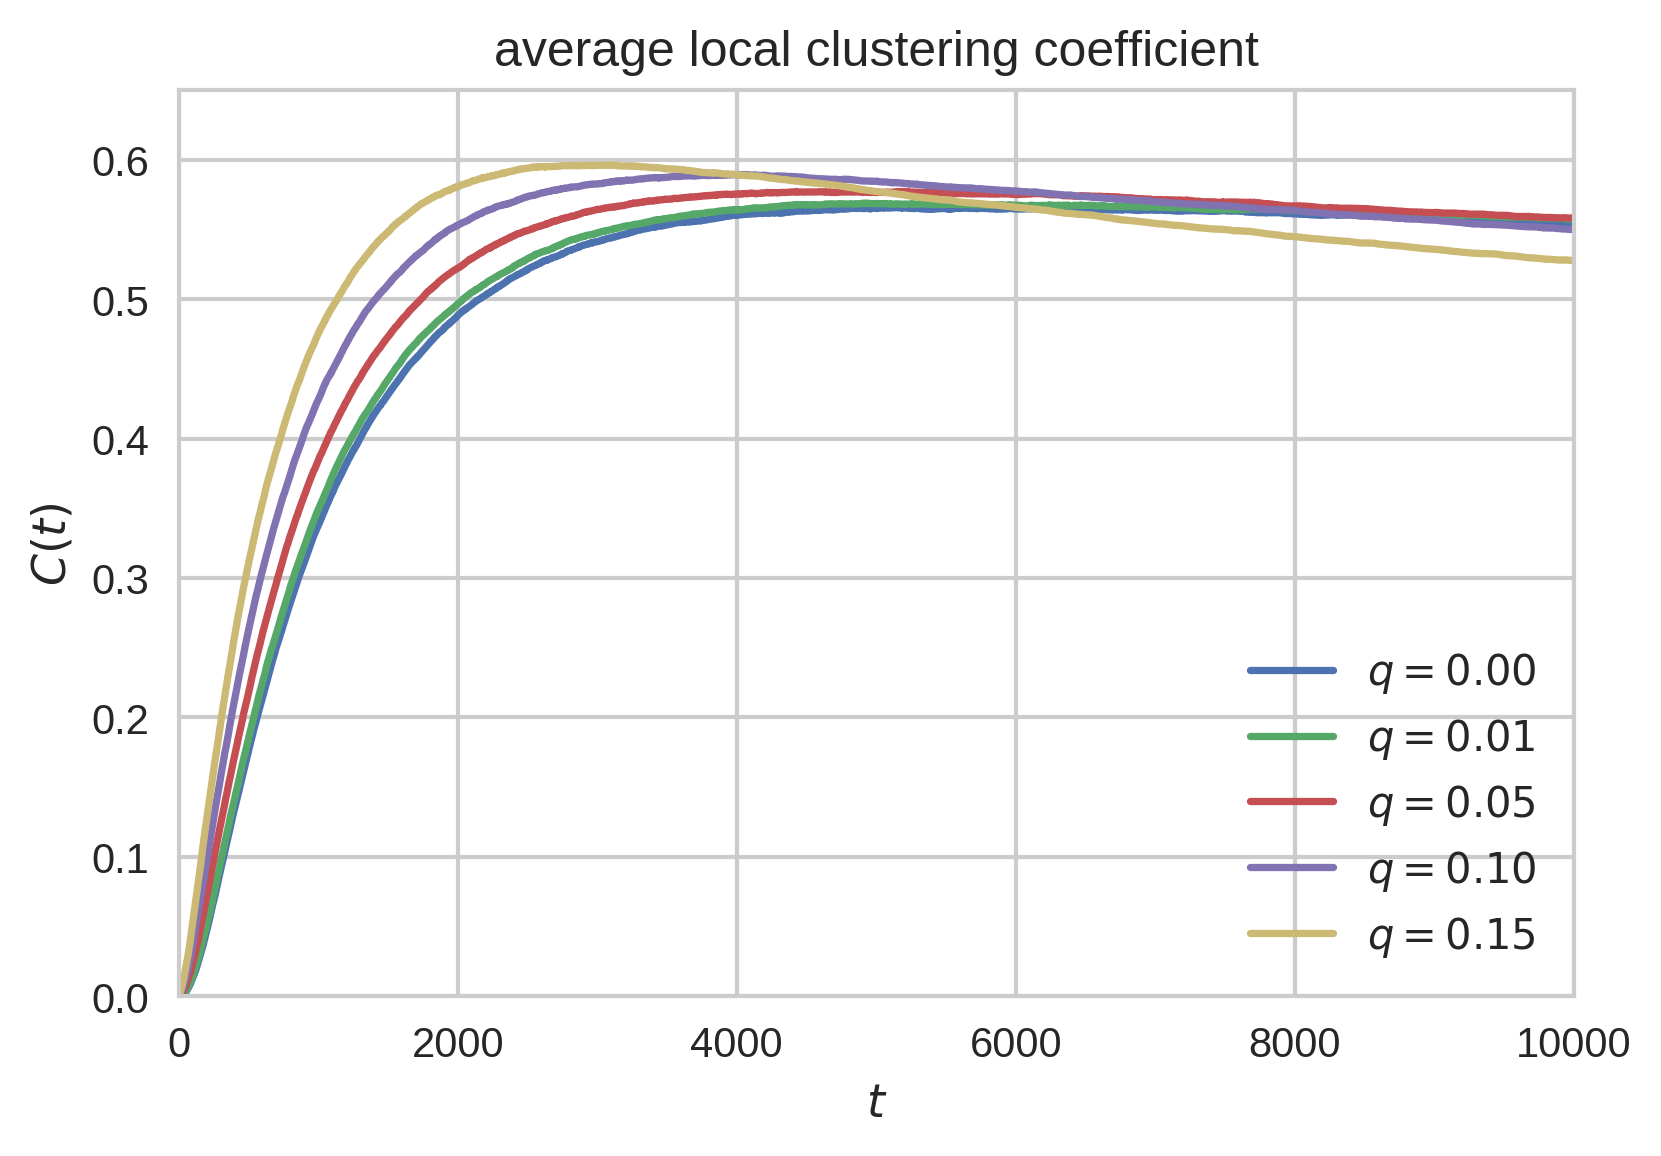
\includegraphics[width=\textwidth]{figures/avg-local-cc-start}
  \caption{}
  \label{fig:avg-local-cc-start}
\end{subfigure}
~
\begin{subfigure}[b]{0.485\textwidth}
  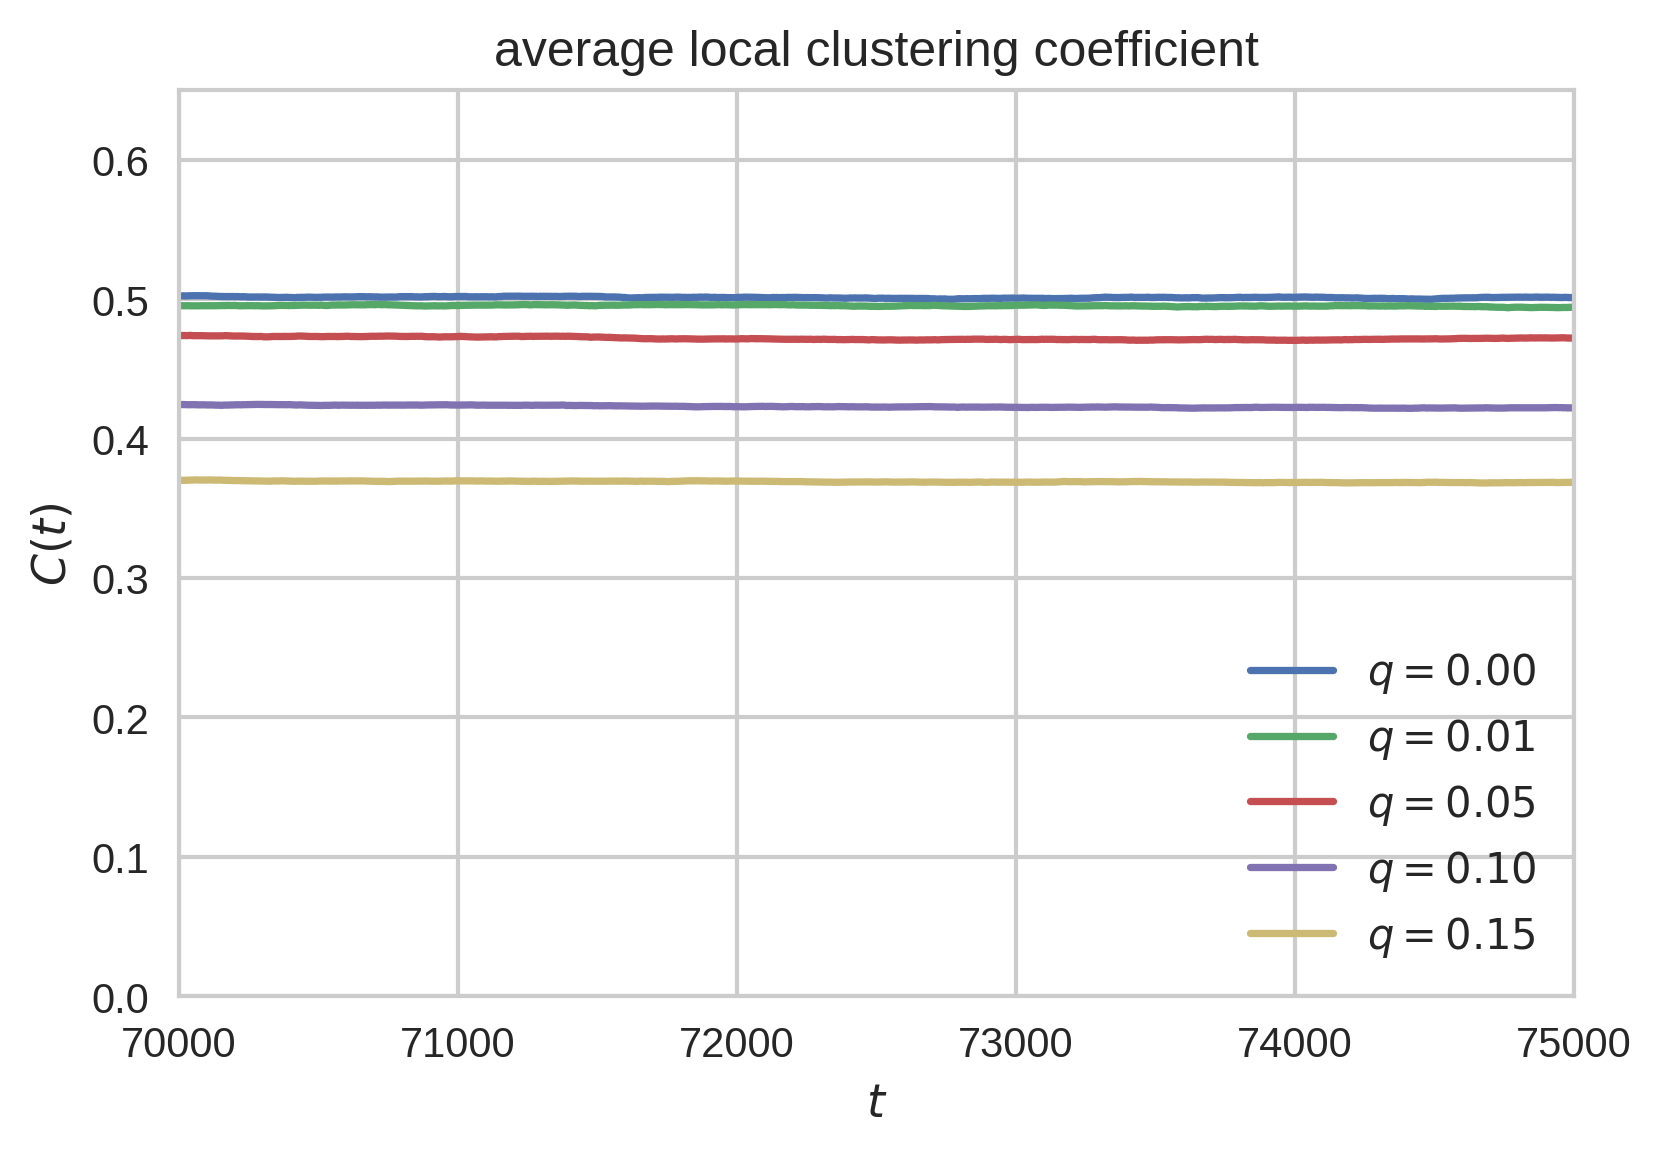
\includegraphics[width=\textwidth]{figures/avg-local-cc-end}
  \caption{}
\label{fig:avg-local-cc-end}
\end{subfigure}

\caption[Segments of the average local clustering coefficient evolution]{Segments of the evolution of the local clustering coefficient for different levels of peer influence. (\subref{fig:avg-local-cc-start}) shows the clustering coefficient for the first 10,000 iterations of the simulation, in which it reaches it maximum value and slowly starts to decrease. (\subref{fig:avg-local-cc-end}) depicts the stationary values for \( C \), which can be observed in the last 5,000 iterations.}
\label{fig:avg-local-cc-details}
\end{figure}


\begin{table}
\centering
\begin{tabular}{llllllll}
\( q \) & 0.00 & 0.01 & 0.025 & 0.05 & 0.075 & 0.10 & 0.15 \\ \hline
\( t_{\max} \) & 5,140 & 4,919 & 4,839 & 5,192 & 4,173 & 4,044 & 3,038 \\ \hline
\( C_{\max} \) & 0.5659 & 0.5689 & 0.5721 & 0.5773 & 0.5822 & 0.5895 & 0.5963
\end{tabular}

\caption[\( \max \) and \( \argmax \) of \( C(t) \)]{The maximum value for the local clustering coefficient \( C_{\max} = \max C(t) \) and the time to reach the maximum \( t_{\max} = \argmax C(t) \), for different values of \( q \).}
\label{tbl:max-clustering}
\end{table}


 The share of reinforcement activity does converge to a value of over 90\% for all levels of peer influence after a short period of time, which highlights the domination of the reinforcement process.
\Cref{fig:percentage-reinforced-ties} shows the plots of the percentage of reinforcement activity for the initial phase of the simulation and over all 75,000 iterations.
The plots of \( r(t) \) also reveal a link between the extent of reinforcement that is happening and the level of peer influence.
In the network with no peer influence effects is the proportion of reinforced to created ties on average 0.8961.
The value increases to 0.9550 in the temporal network with a maximum peer influence probability of 15\%.
This can possibly attributed to the overall increased activity within communities, due to the peer influence effects, and the associated bias towards local strong ties.
With other words, the increased local activity overshadows the introduction of random links by low-activity and/or poorly integrated nodes.


\begin{figure}[htbp]
\centering
\begin{subfigure}[b]{0.485\textwidth}
  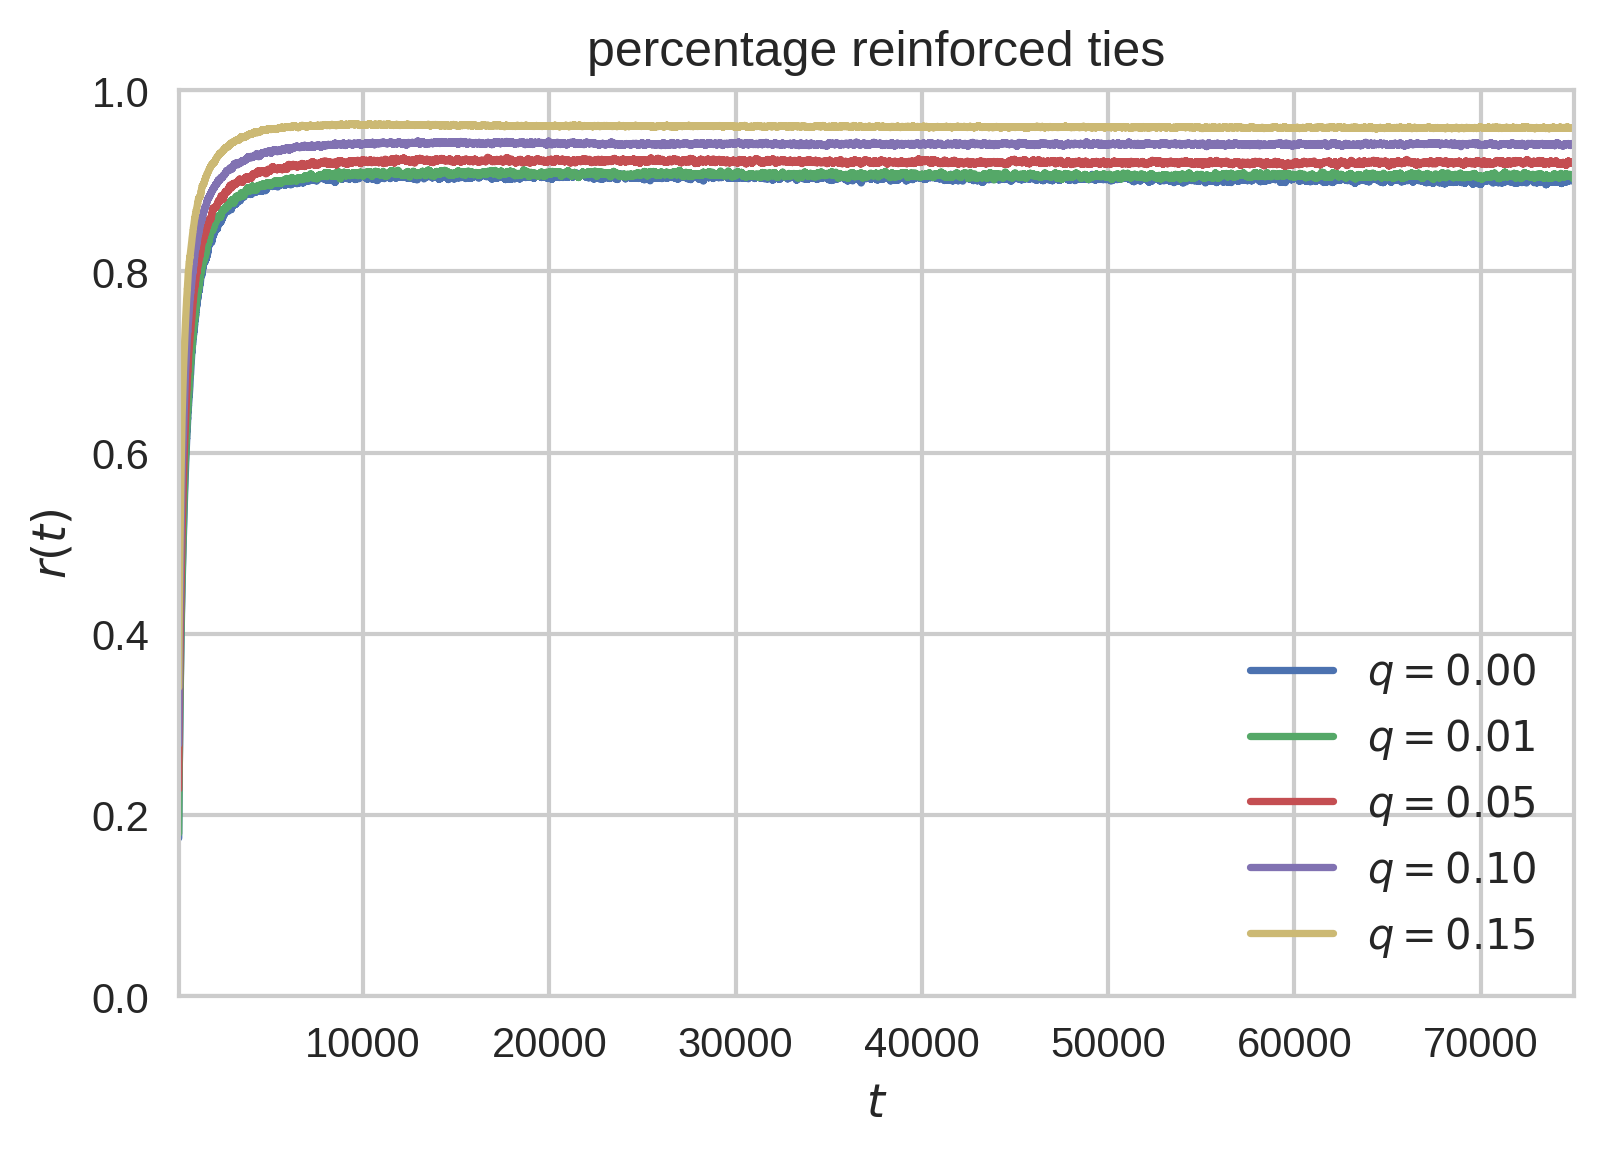
\includegraphics[width=\textwidth]{figures/percentage-reinforced-ties-full}
  \caption{}
  \label{fig:percentage-reinforced-ties-full}
\end{subfigure}
~
\begin{subfigure}[b]{0.485\textwidth}
  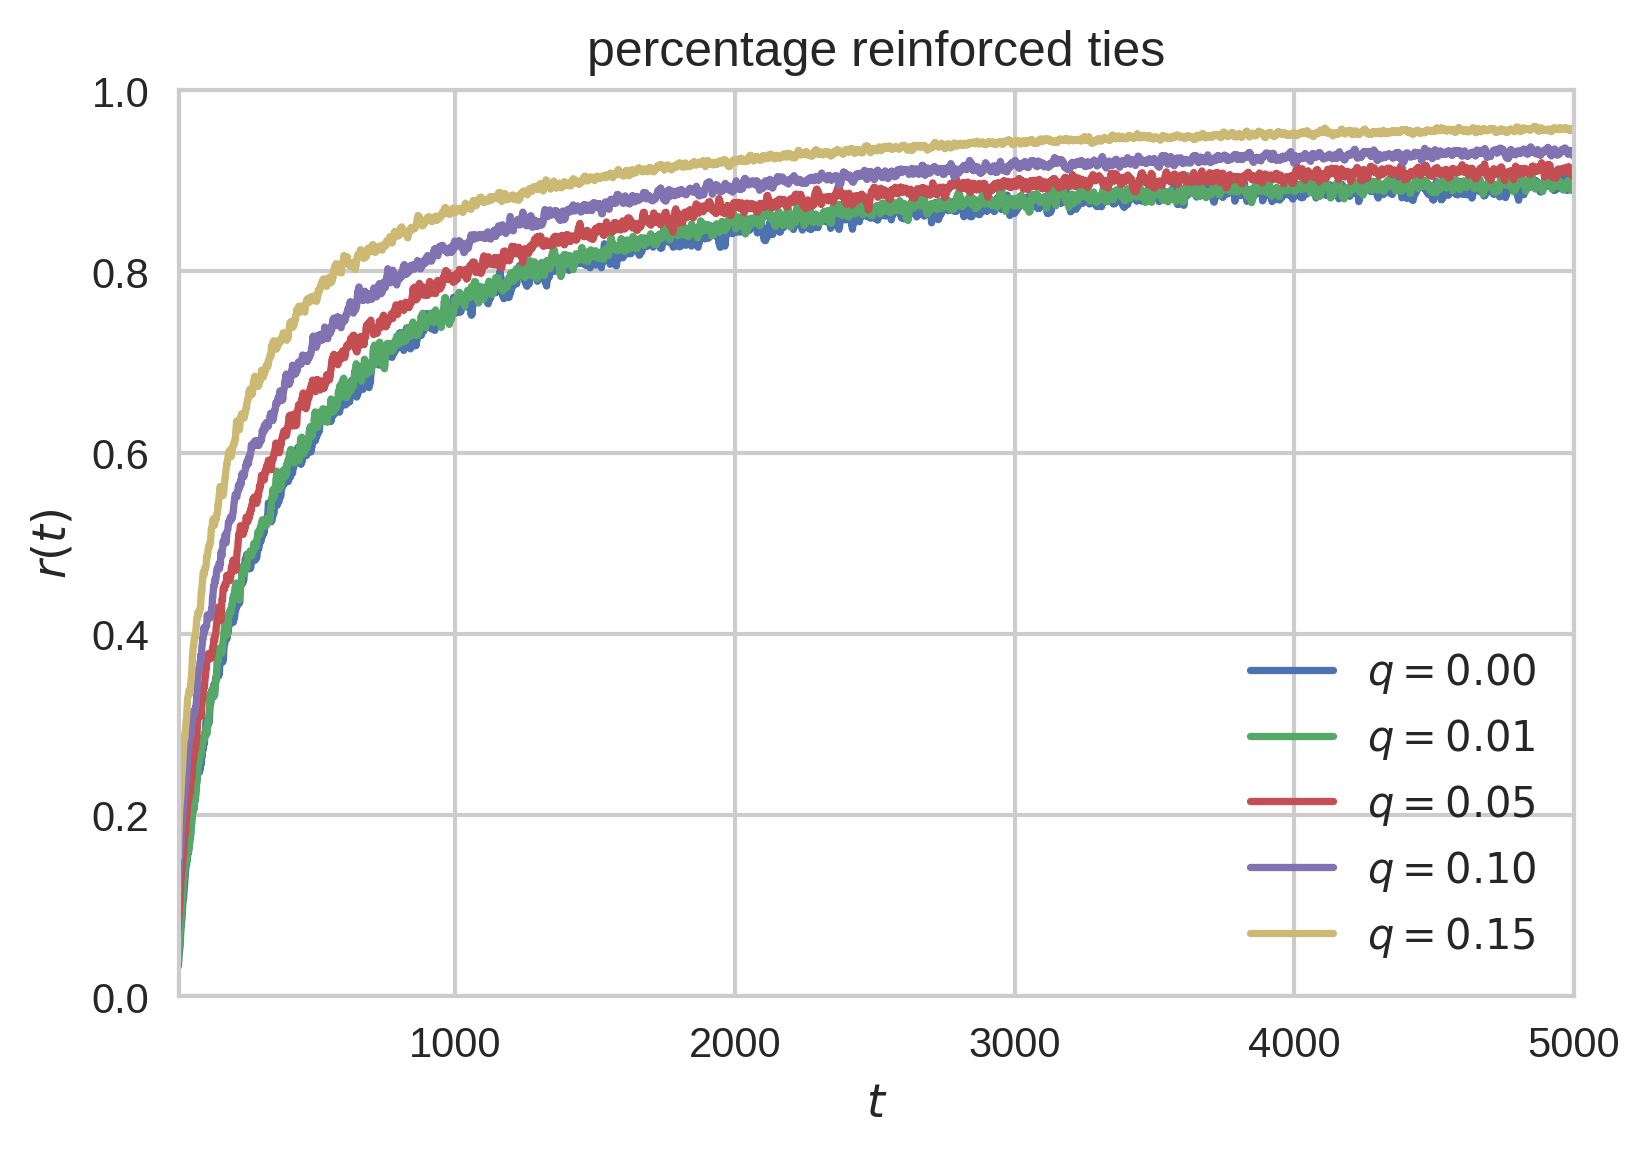
\includegraphics[width=\textwidth]{figures/percentage-reinforced-ties-beginning}
  \caption{}
  \label{fig:percentage-reinforced-ties-beginning}
\end{subfigure}

\caption[Percentage of reinforced ties as function of time]{The percentage of reinforced ties \( r(t) = \frac{\#e_{r}(t)}{\#e_{r}(t) + \#e_{c}(t)} \) for different levels of peer influence as a function of time, where \( \#e_{c}(t) \) and \( \#e_{r}(t) \) are the number of created ties and the number of reinforced ties in iteration \( t \), respectively. (\subref{fig:percentage-reinforced-ties-full}) shows the ratio over all 75,000 iterations and (\subref{fig:percentage-reinforced-ties-beginning}) highlights the behavior in the beginning. Both functions were smoothed using the rolling mean method to improve the quality of the plot.}
\label{fig:percentage-reinforced-ties}
\end{figure}


The evolution of the average local clustering coefficient does dependent on the node deletion probability \( p_{d} \), due to low active nodes which are not removed fast enough and are introducing weak ties~\cite{Laurent2015}.
However, as clearly evident in \cref{fig:avg-local-cc-full}, the possible level of peer influence does influence the clustering, and therefore the community structures of the network, as well.
For example, the more likely an activation due to peer influence gets, the smaller the stationary value for \( C \) becomes.
\Cref{fig:avg-local-cc-end} highlights this effect well.
This can possibly be explained in a similar way as the effect caused by the deletion probability.
However, in this case not the decelerated removal of nodes responsible, but the overall increased activity.
The peer influence mechanism increases the activity in the network, especially in already formed communities (see \cref{sec:network-activity}), since active nodes motivate their neighbors to become active as well.
The probability for the formation of a new tie is inverse proportional to the size of a nodes' egocentric network.
Therefore, a active node which is already fully integrated in its community will reinforce one of its existing ties, or at least close a triangle, with high probability.
However, given enough tries such a node will eventually introduce new weak ties using the focal closure mechanism as well.
Therefore, the opportunities for the introduction of random links by active nodes increases, which leads to a smaller average local clustering in general.

Two additional measures of the integrated network, the average node degree and the average tie strength, were tracked over time for different magnitudes of peer influence as well.
\Cref{fig:avg-weigth-and-tie-strength} depicts the graphs for these two network properties as functions of time.
Both measures show a similar general behavior.
The average degree and the average tie strength are not independent on the maximum peer influence probability in the network and do converge after the integrated network reaches its equilibrium.
The stationary values of both do increase with increasing values for \( q \) by about the same order of magnitude, which is reasonable since both measures are related to each other.
The tie strength of a node can be seen as its weighted degree.
However, the time it takes until they converge differs.
The average degree takes longer to reach its stationary value.
This can be explained by the small probability for the creation of new ties after the egocentric networks have gained a certain size.
Every new neighbor reduces the probability for the creation of new tie in the future significantly.
The average tie strength does not suffer from this problem, due to to fast development of strong ties and the decreasing probability for the introduction of weak ties. \todo{sound explanation?}
The direct effect of the peer influence mechanism on the average degree and average weight can be explained, similar to the average local clustering coefficient, by the additional activity in the temporal network.
The nodes are getting more opportunities to add additional neighbors and to strengthen their ties until they get removed.
Note that the slightly different convergence behavior of the average tie strength for the high peer influence probability \( q = 0.15 \) cannot be explained fully at this point. It may be related to the by comparison significantly slower converge of the average degree, but it is ultimately left open for possible future studies.


\begin{figure}[htbp]
\centering
\begin{subfigure}[b]{0.485\textwidth}
  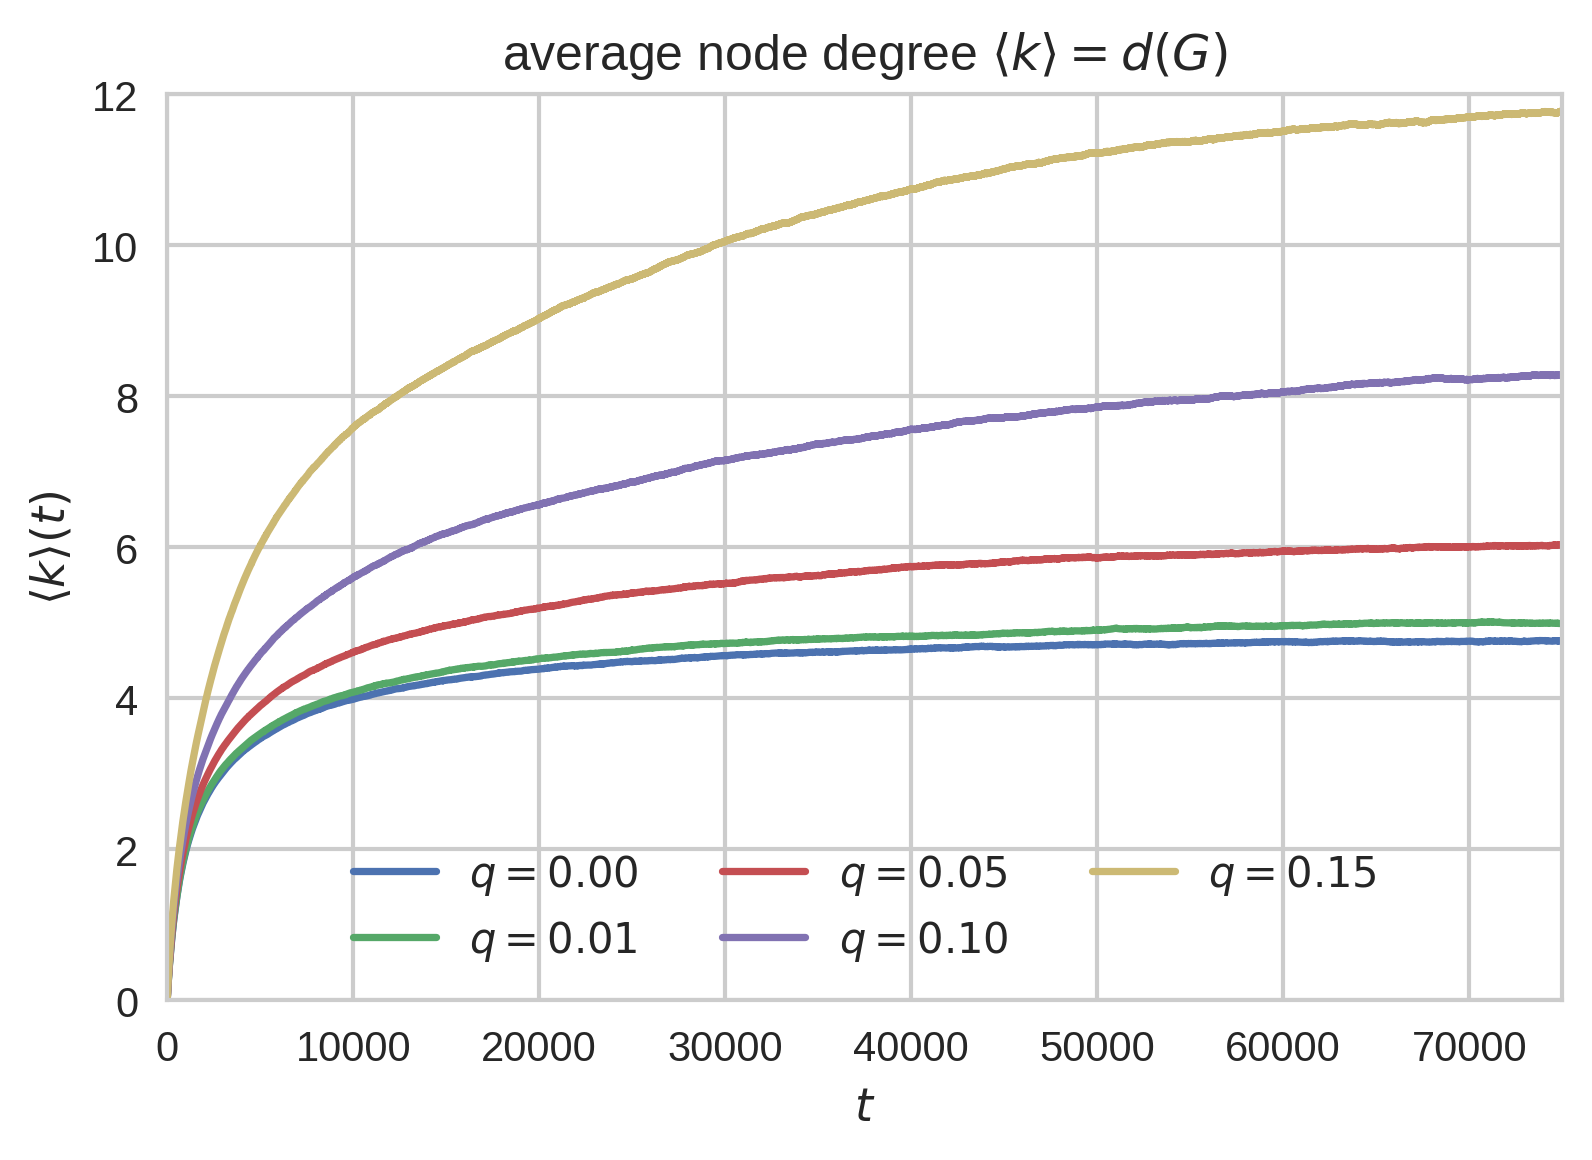
\includegraphics[width=\textwidth]{figures/avg-degree}
  \caption{}
  \label{fig:avg-degree}
\end{subfigure}
~
\begin{subfigure}[b]{0.485\textwidth}
  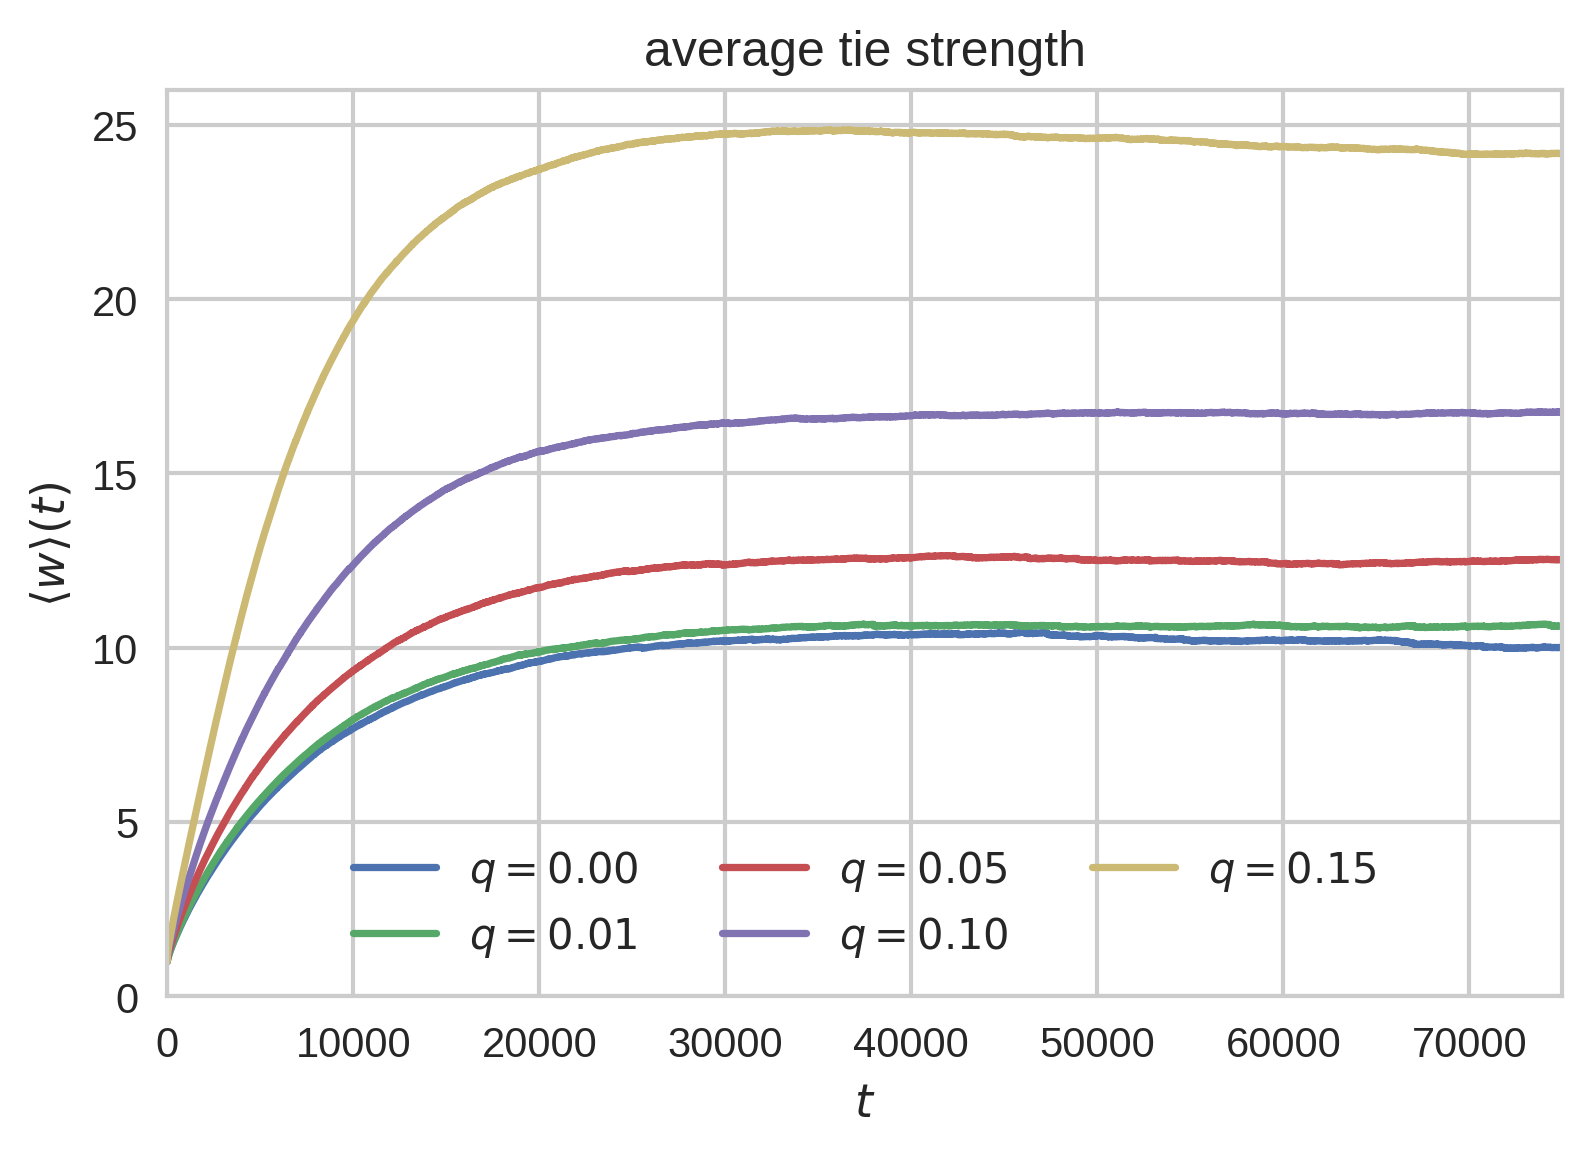
\includegraphics[width=\textwidth]{figures/avg-tie-strength}
  \caption{}
\label{fig:avg-tie-strength}
\end{subfigure}

\caption[Average degree and tie strength as function of time]{Plots of (\subref{fig:avg-degree}) the average node degree \( d(G_{T}) \) and (\subref{fig:avg-tie-strength}) the average tie strength \( \langle w \rangle \) in the network as a function of time for different maximum peer influence probabilities \( q = 0, \, 0.01, \, 0.05, \, 0.1, \, 0.15\). }
\label{fig:avg-weigth-and-tie-strength}
\end{figure}


%% ========================================================================
%% ========================================================================


\section{Network Activity}
\label{sec:network-activity}


\begin{figure}[htbp]
\centering
\begin{subfigure}[b]{0.485\textwidth}
  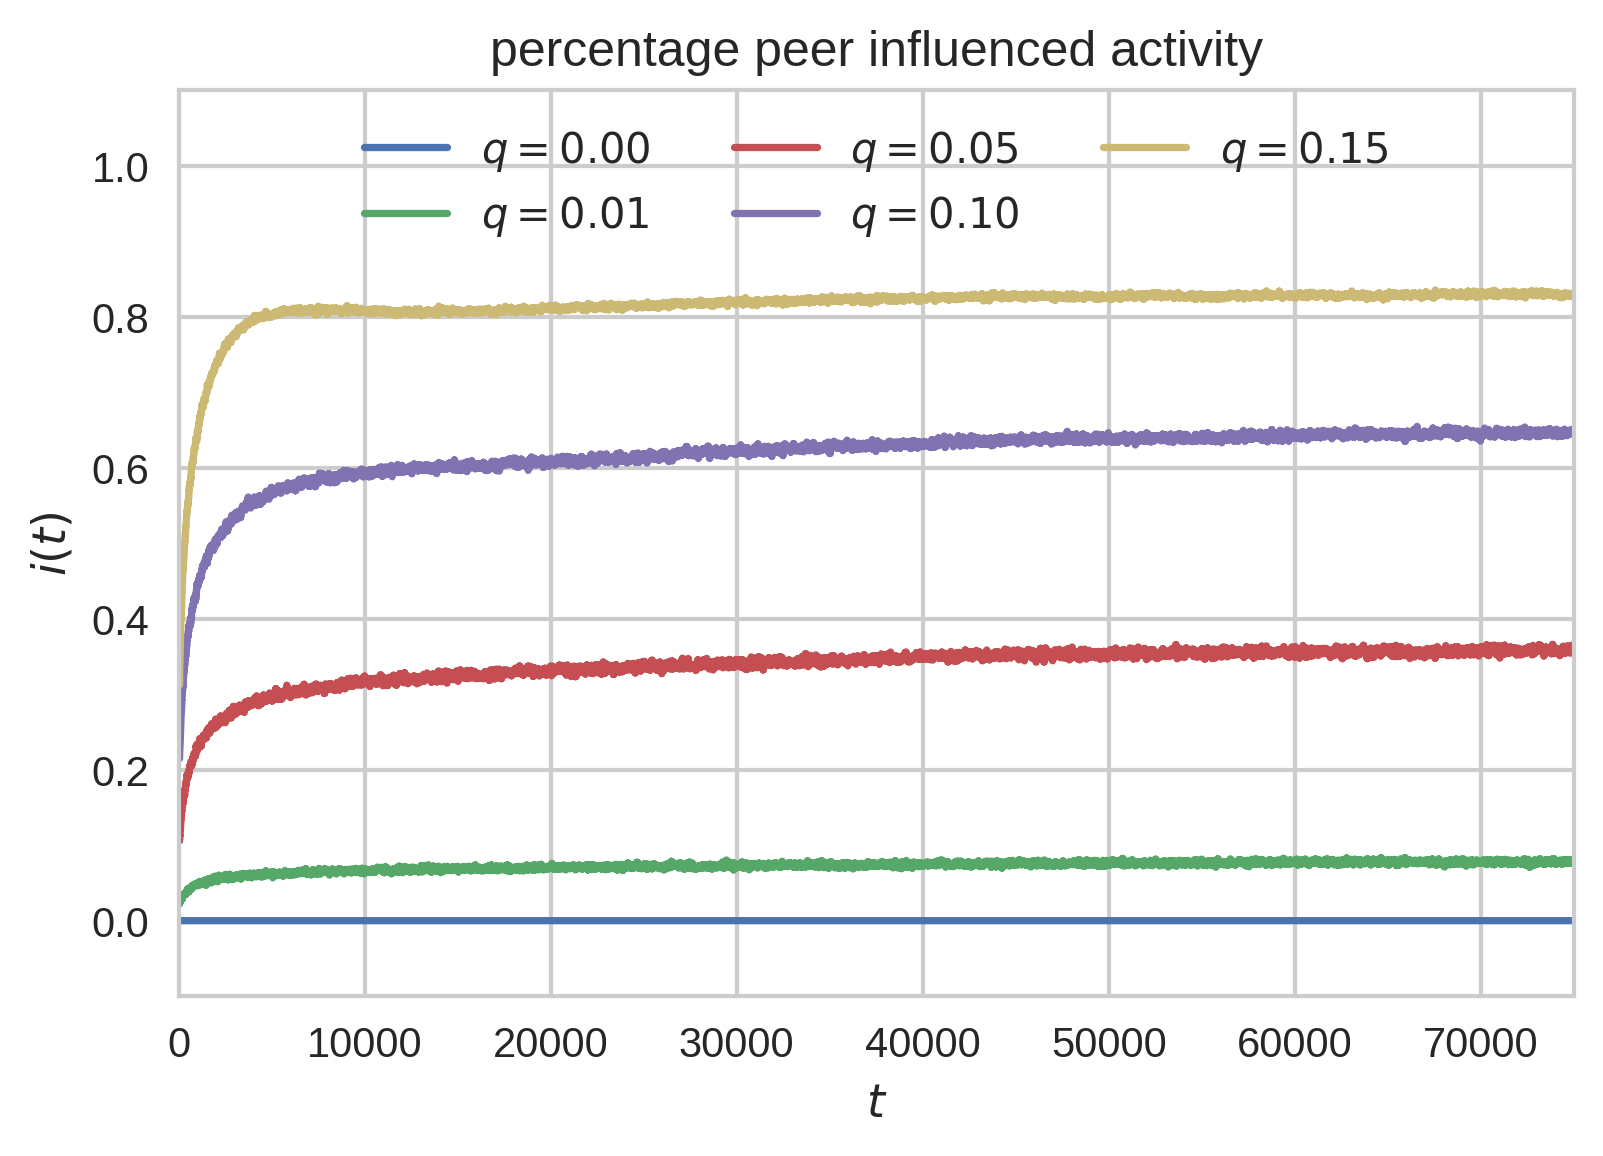
\includegraphics[width=\textwidth]{figures/percentage-influenced-activity-full}
  \caption{}
  \label{fig:percentage-peer-influenced-activity-full}
\end{subfigure}
~
\begin{subfigure}[b]{0.485\textwidth}
  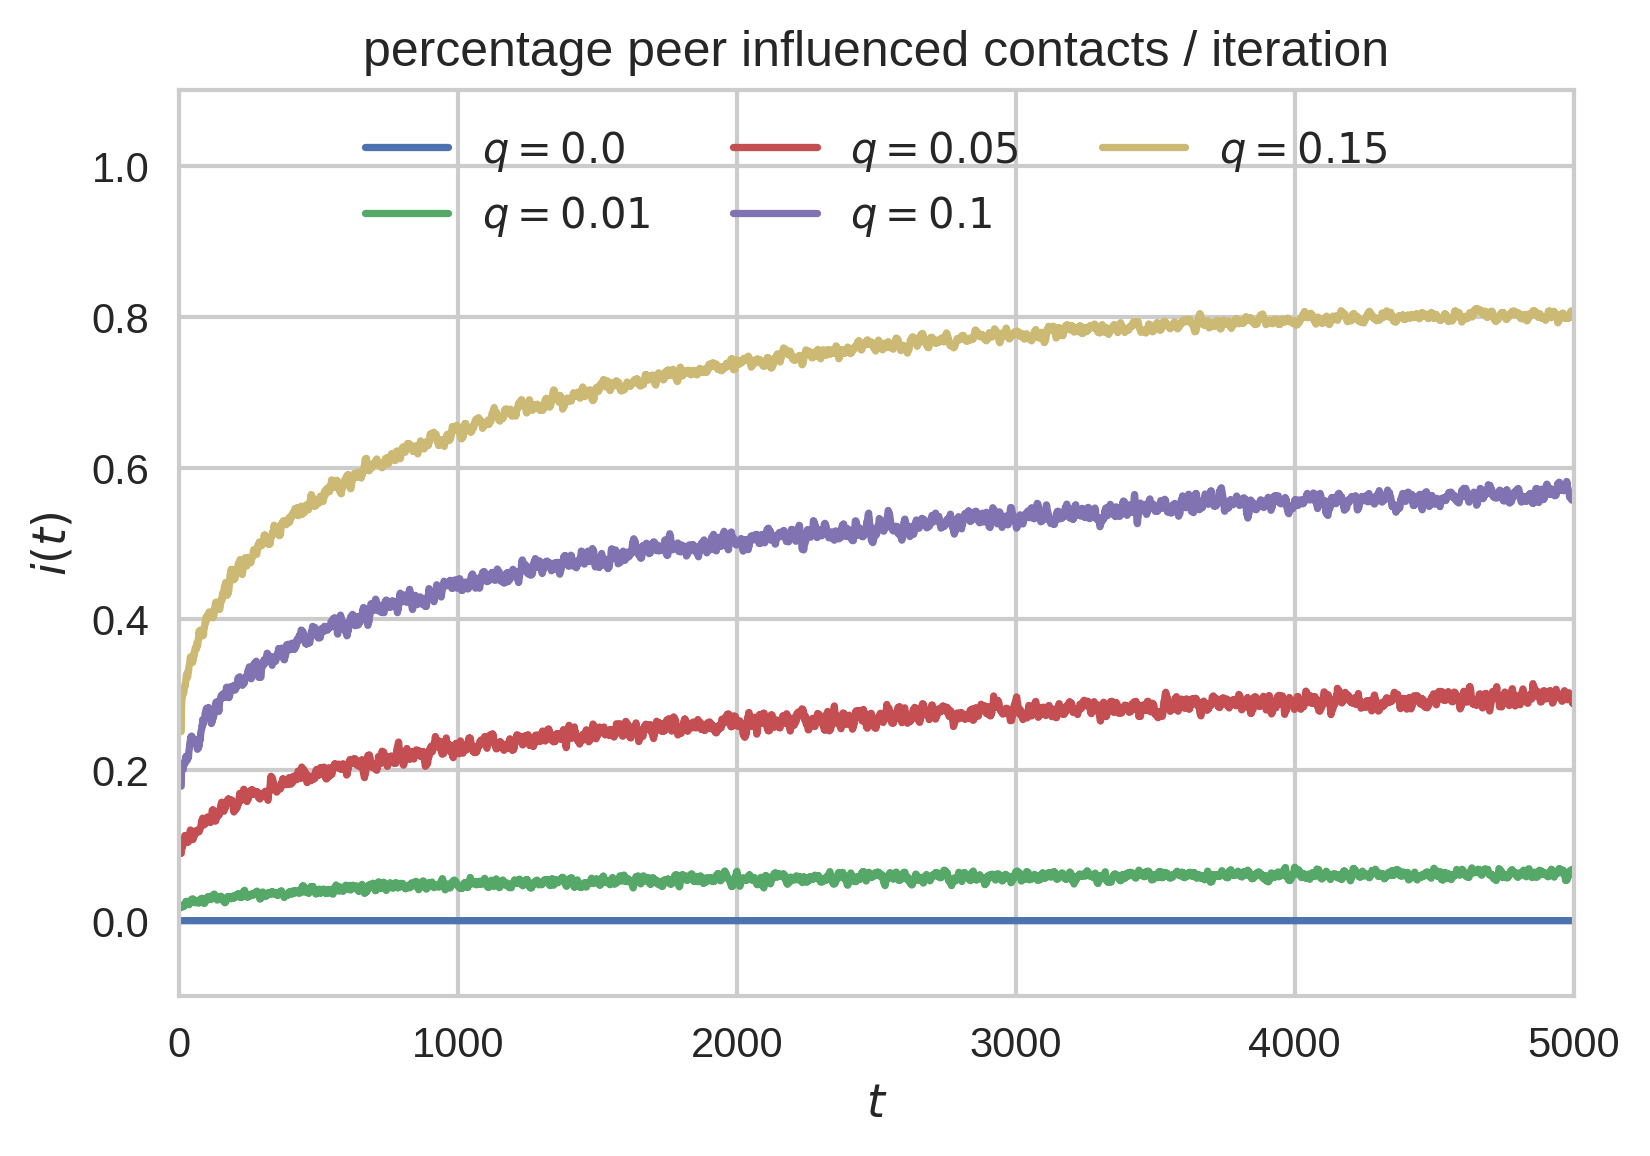
\includegraphics[width=\textwidth]{figures/percentage-influenced-activity-beginning}
  \caption{}
\label{fig:percentage-peer-influenced-activity-beginning}
\end{subfigure}

\caption[Percentage of peer influenced activity as function of time]{Evolution of the fraction of peer influenced activity \( i(t) = \frac{\#e_{p}(t)}{\#e_{p}(t) + \#e_{a}(t)} \) over time for different levels of peer influence, where \( \#e_{p}(t) \) denotes the number of activations caused by peer influence and \( \#e_{a}(t) \) the number of activations due to the intrinsic activity potential at time \( t \), respectively. (\subref{fig:percentage-peer-influenced-activity-full}) shows the ratio over all 75,000 iterations and (\subref{fig:percentage-peer-influenced-activity-beginning}) highlights the behavior in the beginning. Both functions were smoothed using the rolling mean method to improve the quality of the plot.}
\label{fig:percentage-peer-influenced-activity}
\end{figure}


%% ========================================================================
%% ========================================================================


\section{Inter-event Time Distributions}
\label{sec:inter-event-time-dists}
% definition burstiness and parameter B is invariant wrt to activity homogeneity in \cite{Goh2008}
% nice explanation for B in \cite{Masuda2016}


%% ========================================================================
%% ========================================================================


\section{Softmax Weight Re-scaling}
\label{sec:softmax-rescaling}
